\author{João Gonçalves}
\newcommand{\authorr}{Teresa Nogueira}
\newcommand{\authorrr}{André Teodósio}
\newcommand{\authorrrr}{Francisco Carvalho}
\newcommand{\studentID}{99995}
\newcommand{\studentIDD}{100029}
\newcommand{\studentIDDD}{99889}
\newcommand{\studentIDDDD}{99941}
%\newcommand{\supervisorone}{Prof\textsuperscript{\underline{a}}. XXXXXX}
\newcommand{\supervisorone}{Prof. João Silvestre}
\newcommand{\supervisortwo}{}
\newcommand{\department}{Engenharia Eletrotécnica e de Computadores}
\newcommand{\exam}{Modelação e Simulação}

\title{%
Trabalho 2\\
\large Simulação de Monte Carlo do jogo do Monopólio}
\date{Dezembro 2022}

\documentclass[a4paper,12pt]{article}
\usepackage[left=30mm,top=25mm,right=30mm,bottom=25mm]{geometry}
\usepackage[bottom]{footmisc}
\usepackage{etoolbox}
\usepackage{pgfplots}
\usepackage{circuitikz}
\usepackage{booktabs}
\usepackage[usestackEOL]{stackengine}
\usepackage[T1]{fontenc}
\usepackage[utf8]{inputenc}
\usepackage{bm}
\usepackage[export]{adjustbox}
\usepackage{graphicx}
\usepackage[font=footnotesize]{caption}
\usepackage[justification=centering]{subcaption}
\usepackage{amsmath}
\usepackage{amsfonts}
\usepackage{mathtools}
\usepackage{float}
\usepackage[linktoc=all]{hyperref}
\usepackage[capitalise]{cleveref}
\usepackage{enumitem,kantlipsum}
\usepackage[square,numbers,sort]{natbib}
\usepackage[ruled,vlined]{algorithm2e}
\usepackage{listings}
\usepackage[numbered,framed]{matlab-prettifier}
\usepackage{minted}
\usepackage{amssymb}
\usepackage{babel}
\usepackage[nottoc,numbib]{tocbibind}
\usepackage{tcolorbox}
\usepackage{xcolor}
\usepackage{graphicx,array}
\usepackage{breakurl}
\usepackage{placeins}
\usepackage{colortbl}
\usepackage{attrib}
\usepackage{wrapfig}
\usepackage{mathabx}
\usepackage{fancyhdr}
\usepackage{amsmath}
\usepackage[framemethod=TikZ]{mdframed}
%\tcbuselibrary{skins,breakable}
%\usetikzlibrary{shadings,shadows}
\usemintedstyle{emacs}
\linespread{1}
%\setlength{\parindent}{0pt}

\newenvironment{block}[1]{%
    \tcolorbox[beamer,%
    noparskip,breakable,
    colback=LightBlue,colframe=DarkBlue,%
    colbacklower=DarkBlue!75!LightBlue,%
    title=#1]}%
    {\endtcolorbox}

\hypersetup{
    colorlinks,
    linkcolor={black},
    citecolor={blue!50!black},
    urlcolor={blue!80!black}
}

\lstset{
  style              = Matlab-editor,
  basicstyle         = \scriptsize\mlttfamily,
  escapechar         = ",
  mlshowsectionrules = true,
  extendedchars=true,
  literate= {á}{{\'a}}1 {é}{{\'e}}1 {í}{{\'i}}1 {ó}{{\'o}}1 {ú}{{\'u}}1 {ç}{{\c c}}1 {ã}{{\~a}}1 {õ}{{\~o}}1
  {Á}{{\'A}}1 {É}{{\'E}}1 {Í}{{\'I}}1 {Ó}{{\'O}}1 {Ú}{{\'U}}1 {Ã}{{\~A}}1,
}
%//==============================--@--==============================//%
%                   -> reduzir espaço entre itens <-                  %
\usepackage{enumitem}
%\setlist[itemize]{nosep}
%\setlist[enumerate]{nosep}
\setlist[itemize]{itemsep=0.0125em}
\setlist[enumerate]{itemsep=0.0125em}
%//==============================METH-==============================//%
\newcounter{theo}[section]\setcounter{theo}{0}
\renewcommand{\thetheo}{\arabic{theo}}

\definecolor{tempcolor}{RGB}{113, 110, 97}
\newenvironment{theo}[2][]{%
    \refstepcounter{theo}
    \ifstrempty{#1}%
    % if condition (without title)
    {\mdfsetup{%
        frametitle={%
            \tikz[baseline=(current bounding box.east),outer sep=0pt]
            \node[anchor=east,rectangle,fill=blue!20]
            {\strut Teorema~\thetheo};}
        }%
    % else condition (with title)
    }{\mdfsetup{%
        frametitle={%
            \tikz[baseline=(current bounding box.east),outer sep=0pt]
            \node[anchor=east,rectangle,fill=black!20]
            {\strut #1};}%
        }%
    }%
    % Both conditions
    \mdfsetup{%
        innertopmargin=0pt,linecolor=tempcolor,%
        linewidth=2pt,topline=true,%
        frametitleaboveskip=\dimexpr-\ht\strutbox\relax%
    }
 
\begin{mdframed}[]\relax}{%
\end{mdframed}}

\def\delequal{\mathrel{\ensurestackMath{\stackon[1pt]{=}{\scriptstyle\Delta}}}}
%------------------------------------ MAGIC--------------------------------------
\def\UrlBreaks{\do\/\do-}
\expandafter\def\expandafter\UrlBreaks\expandafter{\UrlBreaks\do\a%
\do\b\do\c\do\d\do\e\do\f\do\g\do\h\do\i\do\j\do\k\do\l\do\m\do\n%
\do\o\do\p\do\q\do\r\do\s\do\t\do\u\do\v\do\w\do\x\do\y\do\z\do\&}

\newcolumntype{C}[1]{>{\centering\let\newline\\\arraybackslash\hspace{0pt}}m{#1}}
\newcolumntype{L}[1]{>{\raggedright\let\newline\\\arraybackslash\hspace{0pt}}m{#1}}
%----------------------------------TITLE PAGE -----------------------------------
\makeatletter
\def\maketitle{
  \begin{center}\leavevmode
        \normalfont
        
\includegraphics[width=0.5\columnwidth]{img/title-page/IST.pdf}
        \vskip 0.05cm   
        \textsc{\large \department}\\
        \vskip 0.5cm
        \rule{0.95\linewidth}{0.2 mm} %\\
        {\large \exam}\\[0.5 cm]
        {\huge \bfseries \@title \par} 
        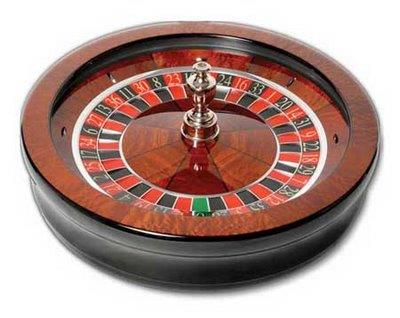
\includegraphics[scale=0.3]{img/title-page/000.jpg}\\
        
\includegraphics[scale=0.35]{img/title-page/001.png}
        \vspace{-0.6em}
        \captionof*{figure}{\color{gray} Imagens: Wikipedia}
        %\vspace{0.5cm}
        \rule{0.95\linewidth}{0.2 mm} \\[0.75 cm]
        %\fontsize{9pt}{11pt}\selectfont
        \begin{minipage}[t]{0.45\textwidth}
	    \begin{flushleft} \large
                \emph{Autores:}\\
		    \normalsize \textbf{\authorrr} : \studentIDDD\\
                \scriptsize $\hookrightarrow$ andre.teodosio@tecnico.ulisboa.pt \\
                \normalsize \textbf{\authorrrr} : \studentIDDDD \\
                \scriptsize $\hookrightarrow$ franciscosoaresc@tecnico.ulisboa.pt
            \end{flushleft}
	\end{minipage}
        \begin{minipage}[t]{0.45\textwidth}
	   \begin{flushleft} \large
                \vphantom{teste 123} \\
			\normalsize \textbf{\@author} : \studentID\\
                \fontsize{9pt}{11pt}\selectfont $\hookrightarrow$ jrazevedogoncalves@tecnico.ulisboa.pt \\
                \normalsize \textbf{\authorr} : \studentIDD\\
                \scriptsize $\hookrightarrow$ maria.teresa.ramos.nogueira@tecnico.ulisboa.pt
		\end{flushleft}
	\end{minipage}
        \vskip 1em
        \begin{minipage}[t]{0.45\textwidth}
	   \begin{flushleft} \large
			\ifdefempty{\supervisortwo}{\emph{Supervisor:\\}}{\emph{Supervisores:\\}}
			\supervisorone\\
			\ifdefempty{\supervisortwo}{}{\supervisortwo\\}
		\end{flushleft}
	\end{minipage}
         \begin{minipage}[t]{0.45\textwidth}
	   \begin{flushright} \large
			\phantom{123 experiência}
		\end{flushright}
	\end{minipage}
        \vspace{0.35cm}
        \begin{quotation}
            \textit{O grupo de alunos acima identificado garante que o texto deste relatório e todo o software e resultados entregues foram inteiramente realizados pelos elementos do grupo, com uma participação significativa de todos eles, e que nenhuma parte do trabalho ou do software e resultados apresentados foi obtida a partir de outras pessoas ou fontes.}
        \end{quotation}
	\vfill
	{\Large \@date\par}
   \end{center}
   %\vfill
   %\null
   \cleardoublepage
  }
\makeatother
%-------------------------------- ENDTITLE PAGE ----------------------------------
%---> Header <---
%\fancyhf{}
\renewcommand{\headrulewidth}{1pt}% Header rule width
\renewcommand{\footrulewidth}{0pt}% No footer rule
\setlength\headheight{26pt} 
\fancyhead[L]{\raisebox{0.1\height}[0pt][0pt]{\textit{Modelação e Simulação}}}
\fancyhead[R]{\raisebox{0.1\height}[0pt][0pt]{2022/2023}}

\pgfplotsset{compat=1.18}
\setcounter{tocdepth}{4}
%\setcounter{secnumdepth}{4}
\setcounter{secnumdepth}{-2}

\renewcommand{\figurename}{Fig.}
\renewcommand{\tablename}{Tab.}
\renewcommand{\contentsname}{Índice}
\settocbibname{Referências}
\setlength{\bibsep}{0.1em}%reduzir espaço entre refs.

\begin{document}
    \sloppy
    %% title page
    \pagenumbering{gobble}
    \maketitle
    %% toc
    %\tableofcontents
    %% body
    \newpage
    \pagestyle{fancy}
    \pagenumbering{arabic}
    \phantomsection\addcontentsline{toc}{section}{Cadeia de Markov}\vskip -0em%
        %//==============================--@--==============================//%
%\vspace{-1em}
\subsection{Introdução}
\label{subsec:intro}

Um dos principais objetivos da análise de Cadeias de Markov, é a determinação das probabilidades de encontrar a cadeia em vários estados, em específicos instantes de tempo. Definimos o \textit{state probability vector} como:
$$
    \pmb{\pi}(k) = [\pi_1(k), \pi_2(k), \pi_3(k), \pi_4(k), \pi_5(k), \pi_6(k), \pi_7(k)]
$$
onde $\pi_j(k) \delequal \mathcal{P}r\{X_k=x_j\}$ no instante $k$, para o espaço de estados $\mathcal{X} = \{x_j\}$, com $j = 1,\dots,7$. E, assim, por associação natural a um sistema dinâmico, a evolução do sistema é dada pela \underline{equação de transição de estados:}
$$
    \pmb{\pi}(k+1) = \pmb{\pi}(k)\, \pmb{P}
$$
em que $\pmb{P}$ é matriz de transição (estocástica) que condensa o comportamento do jogador no tabuleiro consoante o lançamento da moeda.
$$
    \begin{gathered}
        \minipage[c]{\dimexpr0.35\linewidth-2\fboxsep-2\fboxrule\relax}
            \centering
            
\includegraphics[width=0.6\linewidth]{img/Intro/simplifiedMonopoly.png}
            \captionof{figure}{Tabuleiro do Monopólio simplificado. \color{gray} (Imagem: Guia\scalebox{0.7}{$^{*^**}$}).}
        \endminipage
    \end{gathered}
    \qquad
    \pmb{P}=
    \begin{bmatrix}
        0 & 0.5 & 0.5 & 0 & 0 & 0 & 0\\
        0 & 0 & 0.5 & 0.5 & 0 & 0 & 0\\
        0 & 0 & 0 & 0.5 & 0.5 & 0 & 0\\
        0 & 0 & 0 & 0 & 0.5 & 0.5 & 0\\
        0 & 0 & 0.5 & 0 & 0 & 0.5 & 0\\
        0 & 0 & 0.5 & 0 & 0 & 0 & 0.5\\
        0.5 & 0.5 & 0 & 0 & 0 & 0 & 0
    \end{bmatrix}
$$

\noindent $\rightarrow$ \textbf{\textit{Steady-state analysis:}} Qual é a probabilidade de encontrarmos a Cadeia de Markov no estado $x_j$ \textit{"in the long run"\footnotemark[1]}? 
$$ \pi_j = \lim_{k\to+\infty} \pi_j(k) $$
Se $\pi_j$ existir, refere-se como \textit{steady-state}, \textit{equilibrium}, ou \textit{stationary
state probability}. Se existir para todos os estados, definimos o \textit{stationary state probability vector} $\pmb{\pi}$.

\begin{theo}[\underline{Def.:} Irredutibilidade da Cadeia de Markov\protect\cite{Geyer1992}]{def:irredutibilidade}
    A Cadeia de Markov diz-se irredutível sse todos os estados comunicam entre si.
\end{theo}
\vspace{-0.5em}
\begin{theo}[\underline{Def.:} Periodicidade dos estados\protect\cite{Cassandras-Lafortune2008}]{def:periodicidade}
    A periodicidade do estado $x_j\in \mathcal{X}$ é: $\quad d(x_j) \delequal \gcd\{k\in\mathbb{N}^+: \pmb{P}^k(x_j,x_j)>0\} $
    
    \noindent$\rightarrow$ O estado $x_j$ diz-se aperiódico se $d(x_j)=1$ e periódico se $d(x_j)>1$.
\end{theo}
Com base nas definições supramencionadas, invocamos o \textit{\textbf{Ergodic Theorem for Primitive Chains}}\cite{MEDHI2003}, aplicável à Cadeia de Markov objetiva de estudo. \textit{Ergo}, para $k\to+\infty$, $  
\pmb{P}^k \to \pmb{e}\, \pmb{\pi} \implies \pmb{\pi} = \pmb{\pi}\, \pmb{P} \;\land\; \pmb{\pi}\, \pmb{e} = 1$, em que $\pmb{e} = [1\: 1\: 1\: 1\: 1\: 1\: 1]^T$ e $\pmb{\pi}$ pode ser revisto como vetor próprio da matriz estocástica $\pmb{P}$, associado ao valor próprio $\lambda_0 = 1$ ($\rightarrow$ ``\textit{No other eigenvalue of $\pmb{P}$ has absolute value greater than 1.}''\cite{Luenberger1979}).

Justaposto, trivialmente deduzimos (teoricamente) a \textit{equilibrium probability distribution} da Cadeia de Markov em questão:

$$ \therefore \pmb{\pi} = \begin{bmatrix} 0.0455 & 0.0682 & 0.25 & 0.1591 & 0.2045 & 0.1818 & 0.0909 \end{bmatrix} $$
%//==============================--@--==============================//%
\footnotetext[1]{``\textit{By "long run" we mean that the system (...) is allowed to operate for a sufficiently long period of time so that the state probabilities can reach some fixed values (...)}.''\cite{Cassandras-Lafortune2008}}
    \phantomsection\addcontentsline{toc}{section}{Perguntas}\vskip -0em%
        \clearpage
%//==============================--@--==============================//%
%\vspace{-1em}
\subsection{P1 | Distribuição de probabilidades de equilíbrio dos estados do Monopólio simplificado.}
\label{subsec:P1}

%//==============================--A--==============================//%
%\vspace{-0.5em}
\subsubsection{a) Estados percorridos num \textit{run} e valores simulados para o resultado do lançamento da moeda nas sucessivas jogadas desse \textit{run}.}
\label{subsubsec:P1a}

\vspace{-1em}
\begin{figure}[H]
    \centering
    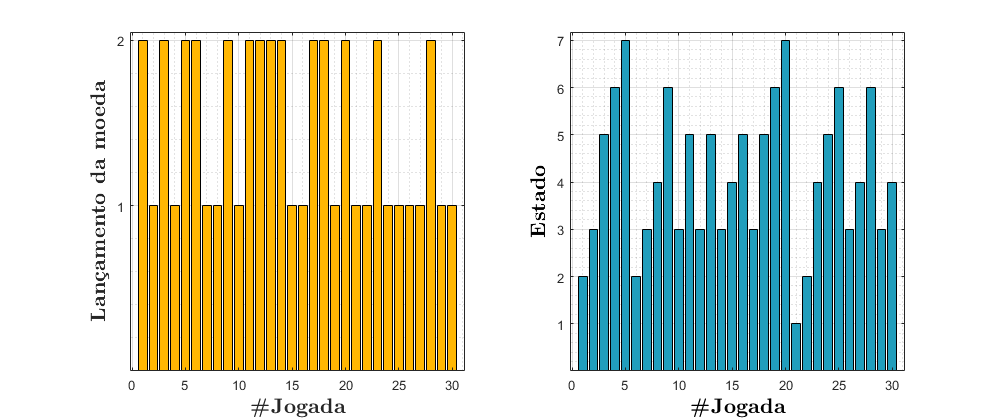
\includegraphics[width = 1\linewidth]{img/P1/P1a.png}
    \caption{Resultado do lançamento da moeda e estados percorridos numa \textit{run} com 30 jogadas\protect\footnotemark[2].}
    \label{fig:P1a}
\end{figure}
\noindent\textbf{\textit{$\rightarrow$ Observações}}

\begin{itemize}
    \item[$\blacktriangle$] O reduzido valor de iterações (jogadas) é escolhido para uma fácil visualização dos gráficos, já que, como veremos em seguida, este valor mostra-se insuficiente para garantir um regime estocástico estacionário.
    \item[$\blacktriangle$] De notar a elevada incidência no estado 3  e 5, resultado congruente com o vetor de equilíbrio (\textit{steady-state vector}) da cadeia em questão (vide \hyperref[subsec:intro]{secção introdutória})
\end{itemize}

%//==============================--A--==============================//%
\footnotetext[2]{Vide \hyperref[subsubsec:P2iii]{secção P2 iii)}.}
%//==============================--A--==============================//%
%//==============================--B--==============================//%
%\vspace{-0.5em}
\subsubsection{b) Frequências relativas dos diferentes estados (muitas jogadas), descartando um transitório inicial.}
\label{subsubsec:P1b}

\vspace{-1em}
\begin{figure}[H]
    \centering
    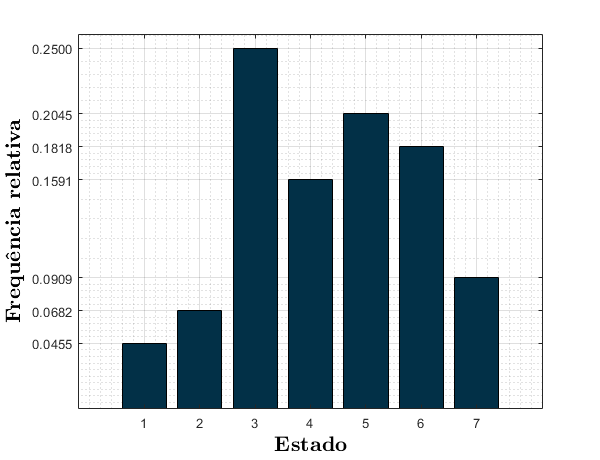
\includegraphics[width = 0.55\linewidth]{img/P1/P1b.png}
    \caption{Frequências relativas para uma simulação de 1000000 \textit{runs} cada uma com 1000 jogadas, de onde 20 são descartadas.}
    \label{fig:P1b}
\end{figure}

\noindent\textbf{\textit{$\rightarrow$ Observações}}
\begin{itemize}
    \item[$\blacktriangle$] Os \textit{steady-state values} simulados de cada estado aproximam-se rigorosamente dos valores teóricos expectáveis (\hyperref[subsec:intro]{secção introdutória}).
    \item[$\blacktriangle$] O valor de \textit{burn-in} (\textit{Ndiscard}) estipulado é o que garante a melhor eliminação do \textit{bias} inicial imposta pela influência da casa de partida ($x_0$).
    \item[$\blacktriangle$] A distribuição das probabilidades estacionárias por estado são intuitivamente explicadas pelo diagrama da cadeia: Sucintamente, $x_1$ é o estado menos provável, a transição (fora a eventual transição inicial do estado $x_0$) só é possível através de uma lançamento com resultado coroa do estado 7. $x_3$ é o estado mais provável, a transição é possível através do estado $x_1$ (coroa), $x_2$ (cara), $x_5$ (coroa) e $x_6$ (cara).   
\end{itemize}


%//==============================--C--==============================//%
%\vspace{-0.5em}
\subsubsection{c) Renda média em regime estocástico estacionário.}
\label{subsubsec:P1c}

Trivialmente se obtêm os valores de renda média efetuando o produto das entradas dos vetores zfreq e Aluguer (nomenclatura conforme o Guia Laboratorial): 
$$ \text{Renda média} = \left[\text{zfreq}(i) \cdot \text{Aluguer}(i)\right]\text{,}\  i = 1, \dots, 7 $$

\vspace{-1em}
\begin{figure}[H]
    \centering
    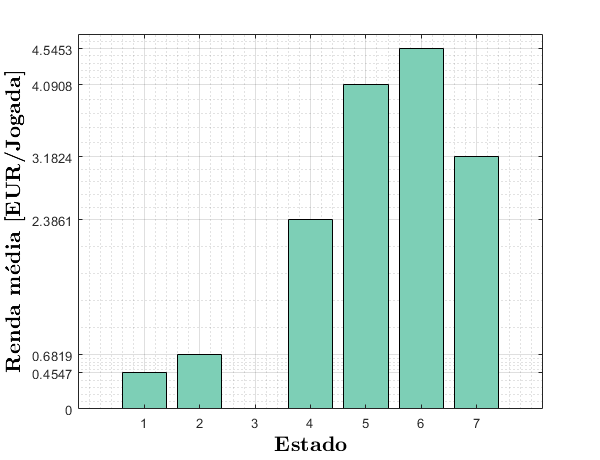
\includegraphics[width = 0.55\linewidth]{img/P1/P1c.png}
    \caption{Renda média para uma simulação de 1000000 \textit{runs} cada uma com 1000 jogadas, de onde 20 são descartadas.}
    \label{fig:P1c}
\end{figure}

\noindent\textbf{\textit{$\rightarrow$ Observações}}
\begin{itemize}
    \item[$\blacktriangle$] O estado 3 possui renda média nula, já que o pagamento é inexistente na prisão (como veremos na \hyperref[subsec:P4]{secção P4} o pagamento poderá equacionar em tempo).
    \item[$\blacktriangle$] A renda é tanto maior quanto maior for a frequência relativa e o preço de aluguer do respetivo estado.
\end{itemize}

%//==============================--@--==============================//%

        %//==============================--@--==============================//%
%\vspace{-1em}
\subsection{P2 | Validação do programa.}
\label{subsec:P2}

%//==============================--A--==============================//%
%\vspace{-0.5em}
\subsubsection{i) Coerência entre a sequência dos estados ao longo das várias jogadas e a sequência de eventos que a determinam.}
\label{subsubsec:P2i}

A transição entre estados depende de um acontecimento definido probabilisticamente (o lançamento da moeda). Complementamos a \hyperref[subsec:intro]{matriz de transição} com a \hyperref[tab:state-transitions]{Tab. 1.:}

\begin{wraptable}[11]{l}{5.5cm}
  \centering
  \label{tab:state-transitions}
  \caption{Transição de estados.}
  \begin{tabular}{ccc}
    \toprule
          & \multicolumn{2}{c}{$\pmb{x_{j+1}}$} \\
    $\pmb{x_j}$ & Cara  & Coroa \\ \midrule
    $x_1$ & $x_2$ & $x_3$ \\
    $x_2$ & $x_3$ & $x_4$ \\
    $x_3$ & $x_4$ & $x_5$ \\
    $x_4$ & $x_5$ & $x_6$ \\
    $x_5$ & $x_6$ & $x_3$ \\
    $x_6$ & $x_3$ & $x_7$ \\
    $x_7$ & $x_1$ & $x_2$ \\ \bottomrule
  \end{tabular}
\end{wraptable}

\noindent $\rightarrow$ \textbf{\textit{Observações}}

\begin{itemize}
    \item[$\blacktriangle$] Afluem quatro estados para $x_3$: 
    \vspace{-0.35em}
    $$ \pi_3 = \dfrac{1}{2}\left(\pi_1 + \pi_2 + \pi_5 + \pi_6\right) $$

    \vspace{-1em}\item[$\blacktriangle$] É apenas possível transitar para os estados $x_2$, $x_4$, $x_5$ e $x_6$ através dos dois estados anteriores:
    \vspace{-1.15em}
    \begin{gather*}
        \pi_2 = \frac{1}{2}(\pi_1 + \pi_7)\qquad\pi_4 = \frac{1}{2}(\pi_2 + \pi_3) \\
        \pi_5 = \frac{1}{2}(\pi_3 + \pi_4)\qquad\pi_6 = \frac{1}{2}(\pi_4 + \pi_5)
    \end{gather*}

    \vspace{-1em}\item[$\blacktriangle$] Transita-se para $x_1$ de $x_7$ e para $x_7$ de $x_6$:
    \vspace{-0.35em}
    $$ \pi_1 = \frac{1}{2}\pi_7 = \frac{1}{2}\left(\frac{1}{2}\pi_6\right) $$
\end{itemize}

A validação dos resultados \hyperref[subsubsec:P1b]{advindos da simulação} e \hyperref[subsec:intro]{deduzidos teoricamente} é naturalmente observada com as relações expostas acima.
%//==============================--A--==============================//%
%\vspace{-0.5em}
\subsubsection{ii) Convergência da distribuição das probabilidades dos diferentes estados com o aumento do número de \textit{runs} de Monte Carlo.}
\label{subsubsec:P2ii}

A convergência da distribuição das probabilidades dos diferentes estados é estudada através do \textit{root mean square error} (\textit{RMSE}) acumulado ao longo de $N$ \textit{runs} de Monte Carlo (NMC)\footnotemark[3]:

%//==============================--A--==============================//%
\footnotetext[3]{Para \textit{runs} de 200 jogadas totais.}
%//==============================--A--==============================//%

\begin{figure}[H] 
    \begin{subfigure}[b]{0.5\linewidth}
        \centering
        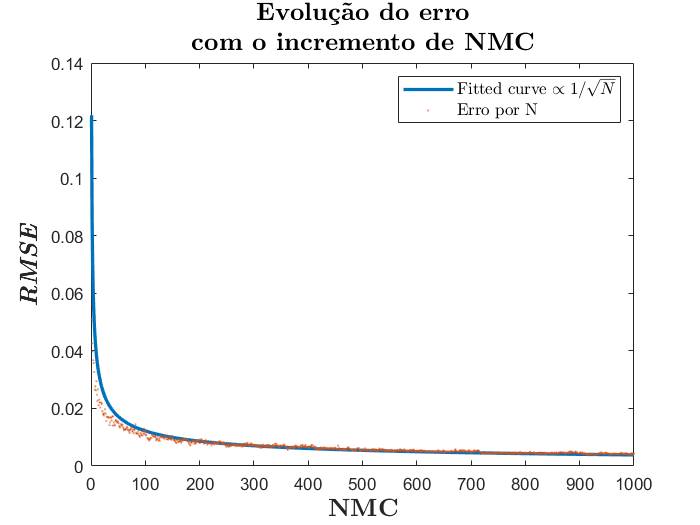
\includegraphics[width=1\linewidth]{img/P2/P2ii-discard.png}
        \caption{Evolução do erro ao longo de N \textit{runs} de Monte Carlo} 
        \label{fig:P2ii} 
        \vspace{1ex}
    \end{subfigure}%% 
    \begin{subfigure}[b]{0.5\linewidth}
        \centering
        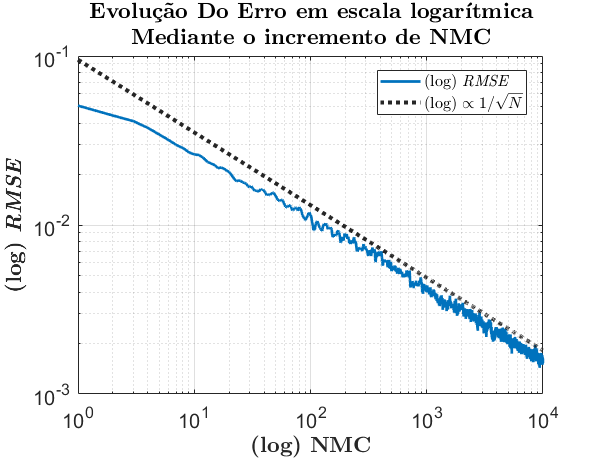
\includegraphics[width=1\linewidth]{img/P2/P2iilog.png} 
        \caption{Evolução do erro em escala logarítmica.} 
        \label{fig:P2ii-log} 
        \vspace{1ex}
    \end{subfigure} 
    \caption{Ilustração da \textit{convergence rate} da Cadeia de Markov.}
\end{figure}

\noindent\textbf{\textit{$\rightarrow$ Observações}}

\begin{itemize}
    \item[$\blacktriangle$] A \textit{fitted curve} demonstra que o decaimento do erro tem um \textit{rate} $\propto\, 1/\sqrt{N}$ (onde $N$ são as \textit{runs} de Monte Carlo) $\rightarrow$ O \textit{convergence rate} dos diferentes estados é da ordem de $\mathcal{O}(1/\sqrt{N})$, realidade independente da dimensão da cadeia:
\end{itemize}
\begin{quote}
    ``Monte Carlo's convergence rate, $\mathcal{O}(1/\sqrt{N})$, is independent of dimension.''\cite{caflisch_2008}
\end{quote}

\begin{itemize}
    \item[$\blacktriangle$] A visualização dos eixos no espaço logarítmico (vide \hyperref[fig:P2ii-log]{Fig. 5 b)}) sugere que para valores elevados de $N$ a aproximação à reta $\propto\: 1/\sqrt{N}$ torna-se cada vez mais refinada.
\end{itemize}

Estudou-se ainda a evolução do erro para \textit{seeds} diferentes, de forma a variar o gerador de números aleatórios:

\begin{figure}[H]
    \centering
    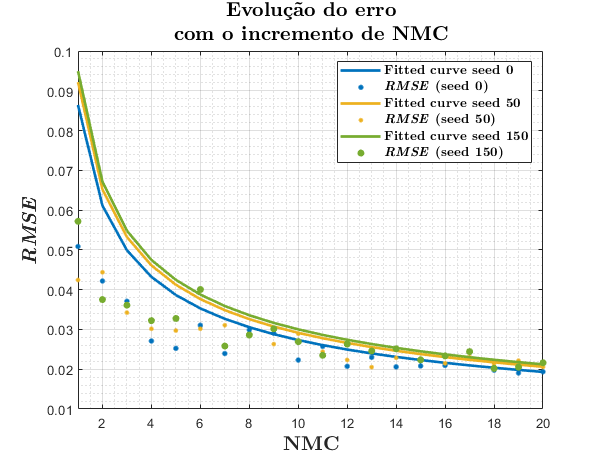
\includegraphics[width = 0.6\linewidth]{img/P2/P2iiseed.png}
    \caption{Convergence rate para \textit{seeds} diferentes.}
    \label{fig:seed}
\end{figure}

\noindent\textbf{\textit{$\rightarrow$ Observações}}

\begin{itemize}
    \item[$\blacktriangle$] A variação do gerador de números aleatórios não afeta a evolução do erro mediante o número de NMC's: as \textit{fitted curves} demonstram sempre que o decaimento do erro tem um \textit{rate} $\propto\: 1/\sqrt{N}$. A não sobreposição aparente das \textit{fitted curves} advém da sequência de números aleatórios distintos, consequentemente, valores de \textit{RMSE} distintos.
\end{itemize}

\vspace{-1.5em}
\subsubsection{iii) Valor adequado da variável Ndiscard.}
\label{subsubsec:P2iii}

\textit{Ndiscard}, normalmente conhecido pelo termo \textit{burn-in}/\textit{warm-up}, destina-se a dar tempo suficiente à Cadeia de Markov para atingir o seu \textit{steady-state}/\textit{equilibrium distribution}, livre do \textit{bias} inicial imposto pelo estado de partida:

\begin{quote}
 \textit{``The idea is that a "bad" starting point may over-sample regions that are actually very low probability under the equilibrium distribution before it settles into the equilibrium distribution. If you throw those points away, then the points which should be unlikely will be suitably rare.''}\cite{amelio}
\end{quote}

Procuramos um número de iterações grande o suficiente para garantir uma cadeia bem misturada, o que se traduz num \textit{RMSE} (\textit{root mean square error}) mínimo:
\newpage
$\rightarrow$ Ao realizar $N$ simulações de Monte Carlo\footnotemark[4], cada uma com \textit{burn-in} incrementalmente diferente, \textbf{pretendemos depreender uma gama de valores de \textit{Ndiscard} para o qual o erro é mínimo e estável.}

\begin{figure}[H]
    \centering
    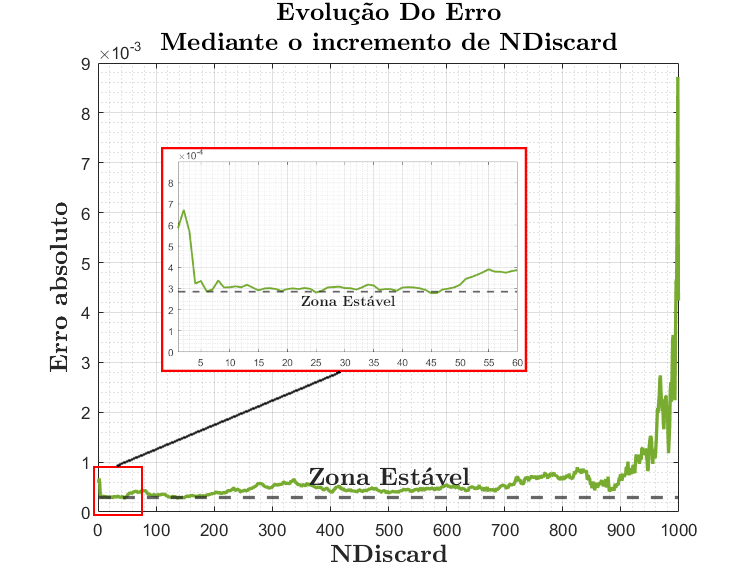
\includegraphics[width = 0.6\linewidth]{img/P2/P2iii.png}
    \caption{Erro absoluto mediante o incremento de \textit{Ndiscard} para simulações de 1000000 \textit{runs} e 1000 jogadas totais. (\textbf{\underline{Nota}:} foi omitido o valor do erro absoluto para \textit{Ndiscard }$= 1000$ de forma a uma melhor visualização do comportamento da evolução do erro. Tal será esperado nas subsequentes figuras.)}
    \label{fig:P2iii}
\end{figure}

\noindent\textbf{\textit{$\rightarrow$ Observações}}

\begin{itemize}
    \item[$\blacktriangle$] Para \textit{Ndiscard} < 5 é identificada uma forte flutuação de erros $\rightarrow$ o regime transitório influência os valores de frequência relativa estimados.
    \item[$\blacktriangle$] Para \textit{Ndiscard} $\in\ ]5, 60]$ o erro calculado atinge uma estabilidade mínima correspondente à gama de valores já supramencionada.
    \item[$\blacktriangle$] Para \textit{Ndiscard} > 60 A regressão do erro torna-se progressivamente maior e mais instável, com um pico na gama $[900,1000[$. Este comportamento é trivialmente explicado pela natureza da Cadeia de Markov: Ao descartar um número de jogadas próximo do seu valor total (1000), a ponderação da probabilidade tem por base um número de amostras reduzido. Reconhecendo que a \textit{equilibrium distribuition} da Cadeia de Markov só é atingida para um elevado valor de transições\footnotemark[5] a estimativa da probabilidade apresenta maior incidência de erro.
\end{itemize}

Por outro lado, a literatura indica que:

\begin{quote}
   \textit{``The amount that should be thrown away is usually less than 1\% of a run whenever a run is long enough to give enough precision. So routinely throwing away the initial 1\% or 2\% of runs will usually suffice.''}\cite{Geyer1992}
\end{quote}

\underline{Logo é admitido um valor ótimo de \textit{Ndiscard} de 20.}
\\\\
\textbf{\textit{$\rightarrow$ Nota:}}
\\
O método de Monte Carlo supõe um elevado número de \textit{runs}\footnotemark[6] para um valor de \textit{Njogadas} satisfatório, podemos ainda admitir o estudo do comportamento do número de erros para duas instâncias diferentes, \textit{Many short runs} e \textit{Few long runs}:

\begin{figure}[H] 
    \begin{subfigure}[b]{0.5\linewidth}
        \centering
        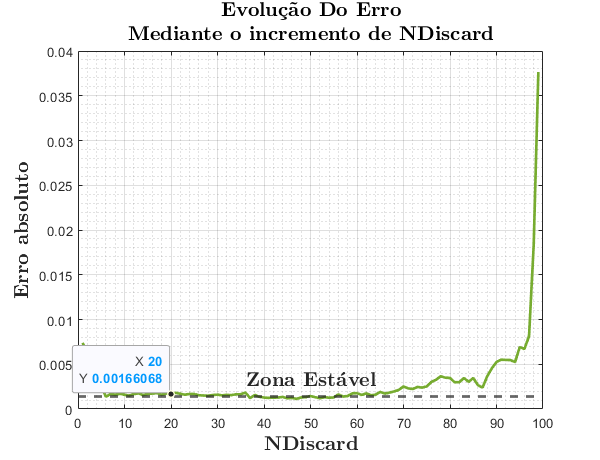
\includegraphics[width=1\linewidth]{img/P2/P2iiishort.png}
        \caption{\textit{Many short runs}:\\ \textit{NMC} = 100000, \textit{Njogadas total} = 100} 
        \label{fig:short} 
        %\vspace{1ex}
    \end{subfigure}%% 
    \begin{subfigure}[b]{0.5\linewidth}
        \centering
        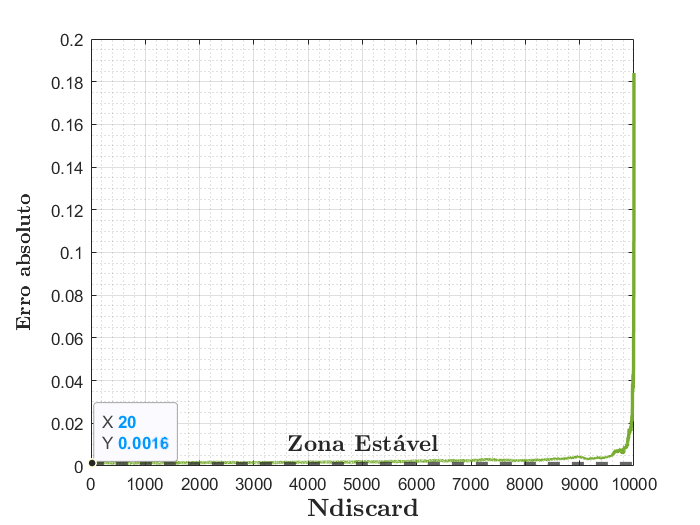
\includegraphics[width=1\linewidth]{img/P2/P2iiilong.png} 
        \caption{\textit{Few long runs}:\\ \textit{NMC} = 100, \textit{Njogadas total} = 100000} 
        \label{fig:Long} 
        %\vspace{1ex}
    \end{subfigure} 
    \caption{Comportamento do número de erros para as duas instâncias.}
    \label{fig:COMPARENdiscard}
\end{figure}

Embora o erro para um \textit{Ndiscard} de 20 seja satisfatório para as duas instâncias já acima referidas é importante compreender que o valor de \textit{burn-in} escolhido é totalmente inerente ao tipo de simulação realizada\footnotemark[7]. Para o P1 são admitidas simulações de 1000000 \textit{runs}, 1000 \textit{Njogadas total} e 20 \textit{Ndiscard} \textbf{(\textit{Many short runs}) já que a \textit{convergence rate} é de $\mathcal{O}(1/\sqrt{N})$ onde $\pmb{N}$ é o número de \textit{runs} de Monte Carlo.}

%//==============================--A--==============================//%
\footnotetext[4]{Entendemos por simulação uma simulação onde decorrem n \textit{runs} de Monte Carlo.}
\footnotetext[5]{Vide \hyperref[subsec:intro]{secção introdutória}.}
\footnotetext[6]{Procuramos simular a Cadeia de Markov NMC (\textit{N de Monte Carlo, número de runs}) vezes.}
\footnotetext[7]{Tipo de Cadeia de Markov, número de \textit{runs} e número de \textit{Njogadas total}.}
%//==============================--A--==============================//%
%\vspace{-0.5em}
\subsubsection{iv) Outros aspetos importantes.}
\label{subsubsec:P2iv}

\noindent\textbf{\textit{$\rightarrow$ Métodos de diagnóstico}}\\
Na literatura, a estimação do \textit{burn-in}/\textit{warm-up}, bem como, da região de convergência da Cadeia de Markov é efetuada mediante diversos padrões de diagnóstico, tais como: \textit{trace plot}, \textit{autocorrelation}... Infelizmente não abordados, devido à \textit{scope} do problema.

\vspace{1em}
\noindent\textbf{\textit{$\rightarrow$ Fórmulas de erro escolhidas}}
\begin{align*}
    \text{RMSE}&\delequal \; \sqrt{\frac{1}{\text{NMC}}\sum\limits_{n=1}^{\text{NMC}}\left\parallel\pmb{\hat{\pi}}_n - \pmb{\pi}_{\text{teo.}}\!\right\parallel} \\
    \text{Erro absoluto}&\delequal \; \sum\limits_{j=1}^{\text{Ncasas}} \left\vert \hat{\pi}_j - \pi_{\text{teo.},j} \right\vert
\end{align*}

O \textit{RMSE} foi escolhido para visualizar a \textit{convergence rate} da distribuição das probabilidades dos diferentes estados dado que pode ser visto como a distância (assemelhando-se à Euclidiana, mas \textit{rescaled}/\textit{normalized}) entre o vetor simulado e o \hyperref[subsec:intro]{vetor teórico esperado}.

O erro absoluto propiciou uma melhor visualização da região de transição prevista na evolução do erro mediante o incremento de \textit{Ndiscard}.
%//==============================--@--==============================//%
        \clearpage
%//==============================--@--==============================//%
%\vspace{-1em}
\subsection{P3 | Probabilidade de estar no estado 4 ao longo das sucessivas jogadas.}
\label{subsec:P3}
A evolução da probabilidade do estado $4$ é avaliada para um valor fixo de \textit{Njogadas} (50) e um valor sucessivamente maior de \textit{runs} de Monte Carlo:

\begin{figure}[ht] 
    \begin{subfigure}[b]{0.5\linewidth}
        \centering
        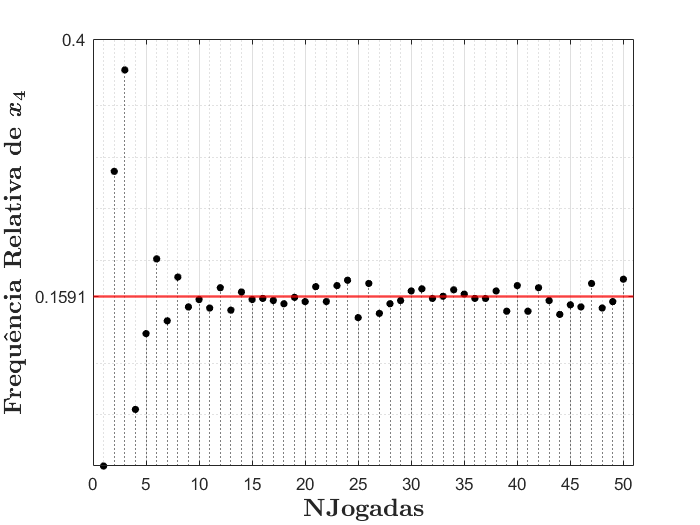
\includegraphics[width=1\linewidth]{img/P3/P31000.png}
        \caption{NMC = 1000} 
        \label{fig:P31000} 
        \vspace{1ex}
    \end{subfigure}%% 
    \begin{subfigure}[b]{0.5\linewidth}
        \centering
        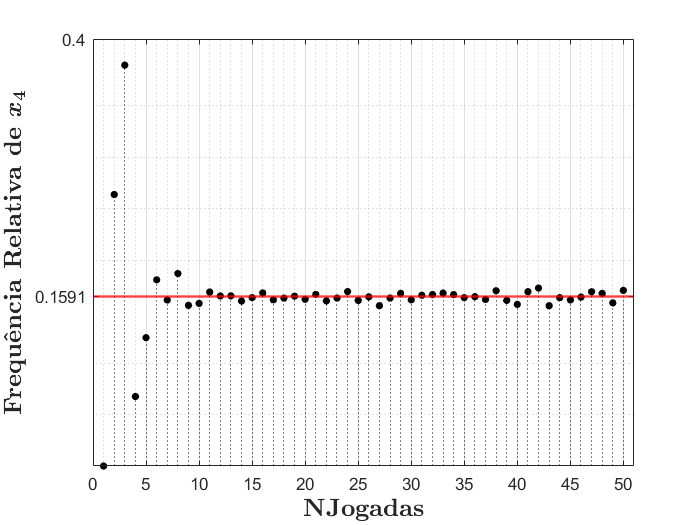
\includegraphics[width=1\linewidth]{img/P3/P310000.png} 
        \caption{NMC = 10000} 
        \label{fig:P310000} 
        \vspace{1ex}
    \end{subfigure} 
    \begin{subfigure}[b]{0.5\linewidth}
        \centering
        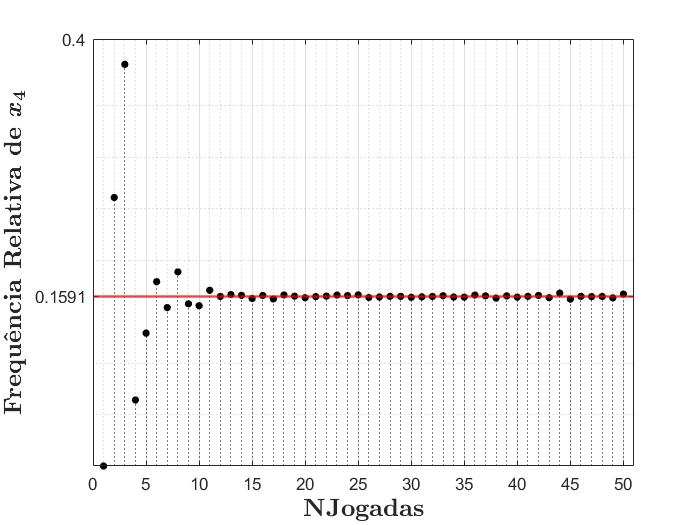
\includegraphics[width=1\linewidth]{img/P3/P3100000.png}
        \caption{NMC = 100000} 
        \label{fig:P3100000} 
        %%\vspace{4ex}
    \end{subfigure}%% 
    \begin{subfigure}[b]{0.5\linewidth}
        \centering
        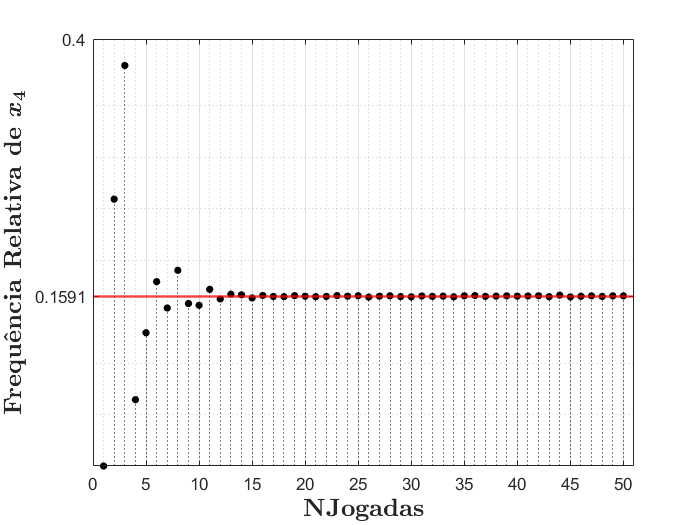
\includegraphics[width=1\linewidth]{img/P3/P31000000.png} 
        \caption{NMC = 1000000} 
        \label{fig:P31000000} 
        %%\vspace{4ex}
    \end{subfigure} 
    \caption{Evolução da probabilidade do estado $4$}
    \label{fig:LABEL}
\end{figure}

\noindent\textbf{\textit{$\rightarrow$ Observações}}

\begin{itemize}
    \item[$\blacktriangle$] Para a primeira jogada a probabilidade de estar no estado 4 é sempre nula, condição imposta pela casa de partida (apenas é possível transitar para o estado 1 ou 2).
    
    \item[$\blacktriangle$] A convergência da probabilidade para o seu \textit{steady-state value} é tanto mais rápida e mais exata quanto maior for o número de \textit{runs} de Monte Carlo (relembramos o \textit{convergence rate} de $\mathcal{O}(1/\sqrt{N})$, vide \hyperref[subsubsec:P2ii]{secção P2 ii)}.
    
     \item[$\blacktriangle$] O número de \textit{Njogadas} não necessita de ser muito grande para atingir uma boa estimativa do \textit{steady-state value}, sendo o número de \textit{runs} o parâmetro de maior peso nesta tarefa, reforçando novamente o uso de \textit{Many short runs}.
\end{itemize}

%//==============================--@--==============================//%
        \clearpage
\usetikzlibrary{automata, arrows.meta, positioning}
%//==============================--@--==============================//%
%\vspace{-1em}
\subsection{P4 | Diagrama de transição modificado.}
\label{subsec:P4}

De modo a emular a permanência no estado prisão durante uma jogada, acrescenta-se um estado \textit{dummy}, denomidado por $x_P$, para o qual se transita, (possivelmente) dos estados $5$ ou $6$. Nestes moldes, uma jogada é desperdiçada entre a transição obrigatória do estado $x_P$ para o estado $3$ (transição esta \underline{independente do resultado do lançamento da moeda}).

\begin{figure}[H]
    \centering
    \begin{tikzpicture}[node distance = 2.7cm, on grid, auto, transform shape]
    
        \node (1) [state, scale=0.8, transform shape] {$x_1$};
        \node (2) [state, above = of 1, scale=0.8, transform shape] {$x_2$};
        \node (3) [state, right = of 2, scale=0.8, transform shape] {$x_3$};
        \node (4) [state, right = of 3, scale=0.8, transform shape] {$x_4$};
        \node (5) [state, below = of 4, scale=0.8, transform shape] {$x_5$};
        \node (6) [state, below = of 5, scale=0.8, transform shape] {$x_6$};
        \node (7) [state, below = of 1, scale=0.8, transform shape] {$x_7$};
        \node (8) [state, left = of 6, scale=0.8, transform shape] {$x_P$};
    
        \path [-stealth, thick]
            (1) edge node [left, rotate=90, xshift=0.35cm, yshift = 0.25cm, transform shape] {\scriptsize Cara} (2)
            (2) edge node [above, transform shape] {\scriptsize Cara} (3)
            (3) edge node [above, transform shape] {\scriptsize Cara} (4)
            (4) edge node [above right, rotate=-90, xshift=-0.5cm, transform shape] {\scriptsize Cara} (5)
            (5) edge node [above right, rotate=-90, xshift=-0.5cm, transform shape] {\scriptsize Cara} (6)
            (6) edge [bend left = 30, transform shape] node [below, transform shape] {\scriptsize Coroa} (7)
            (7) edge node [left, rotate=90,xshift=0.35cm, yshift = 0.25cm, transform shape] {\scriptsize Cara} (1)
            (1) edge [bend left = 30, transform shape] node [below right] {\scriptsize Coroa} (3)
            (2) edge [bend left = 30, transform shape] node [above] {\scriptsize Coroa} (4)
            (3) edge [bend left = 30, transform shape] node [below left] {\scriptsize Coroa} (5)
            (4) edge [bend left = 30, transform shape] node [above right, rotate=-90, xshift = -0.5cm] {\scriptsize Coroa} (6)
            (7) edge [bend left = 30, transform shape] node [above left, rotate=90, xshift=0.5cm] {\scriptsize Coroa} (2)
            (5) edge [bend left = 30, transform shape] node [above left] {\scriptsize Coroa} (8)
            (6) edge node [below left, xshift=0.4cm] {\scriptsize Cara} (8)
            (8) edge node [left] {X} (3);
            
    \end{tikzpicture}
    \caption{Diagrama de transição de estados modificado com a introdução de um \textit{dummy state}, de modo a descartar uma possível jogada, na eventualidade do jogador ser enviado para a prisão.}
    \label{fig:P4}
\end{figure}

Seguindo o mesmo raciocínio, é trivialmente generalizado o esquema para um número arbitrário de jogadas em que se pretende que o jogador permaneça no estado prisão. Esta façanha é concretizável introduzindo os \textit{dummy states} desejáveis entre o estado $x_p$ e o estado $3$, de forma a gastar jogadas com estas transições impostas (sempre \underline{independentes do lançamento da moeda}). 

\iffalse
\noindent Complementa-se o diagrama com a matriz de transição $\pmb{P}$ respetiva:
$$
\pmb{P}=
    \begin{bmatrix}
        0 & 0.5 & 0.5 & 0 & 0 & 0 & 0 & 0\\
        0 & 0 & 0.5 & 0.5 & 0 & 0 & 0 & 0\\
        0 & 0 & 0 & 0.5 & 0.5 & 0 & 0 & 0\\
        0 & 0 & 0 & 0 & 0.5 & 0.5 & 0 & 0\\
        0 & 0 & 0 & 0 & 0 & 0.5 & 0 & 0.5\\
        0 & 0 & 0 & 0 & 0 & 0 & 0.5 & 0.5\\
        0.5 & 0.5 & 0 & 0 & 0 & 0 & 0 & 0\\
        0 & 0 & 1 & 0 & 0 & 0 & 0 & 0
    \end{bmatrix}
$$
\fi
%//==============================--@--==============================//%
    
    %% refs
    %\clearpage
    \bibliographystyle{unsrtnat}
    \nocite{*}
    {\footnotesize%
    \bibliography{refs}}
    %% attachments
    %\newpage
    %\input{appendix.tex}

\end{document}
